\chapter{Individual based approach}
An individual based approach models a problem by analysing the interactions
between discrete entities. Applying this approach to the problem of solute
transport, the entities represent the particles of the solute. The physical
interaction of the particles with each other gives rise to macroscopic phenomena
such as diffusion. The particle-scale interactions are modelled by a set of
\emph{events}, which are problem specific. Once the microscopic properties of a
an individual based model have been specified, it is possible to create
realisations of the system using a stochastic simulation algorithm --- for
example, the Gillespie algorithm (described below). The model
is random in nature, with the events being randomly selected from an appropriate
probability distribution. As such, in order to find the statistical properties
of the system, an ensemble of realisations can be created from which properties
can be estimated. In addition to this, we can make theoretical predictions (in
some cases, exact expressions, and in others, approximations) of the statistical
properties of an individual based system. These are typically derived from a
Master equation, which describes the time evolution of the probability
distribution defining the system.

The two main types of randomness in individual based models are
\begin{itemize}
    \item Intrinsic noise --- randomness arising from the stochastic nature of the
        physical problem;
    \item Quenched disorder --- randomness of a parameter of the system which is
        usually chosen and fixed before allowing the system to evolve.
\end{itemize}
In solute transport in a disordered medium, a source of quenched disorder is the
randomness of the sink locations.
\todo{elaborate?}

We are interested in macroscopic features of the system, including their
statistics, which arise from the both types of disorder and their interactions.

\section{Problem formulation}
In one dimension, we formulate the problem by discretising space into a
finite set of locations at equal intervals. To each spatial location (``urn'') we assign
a non-zero number of particles and particles can move from one urn to
another according to the set of events.

\begin{figure}[ht!]
    \centering
    \psfragfig[width=0.6\textwidth]{individual/figures/urns}
    {
        \psfrag{1}{\(1\)}
        \psfrag{2}{\(2\)}
        \psfrag{3}{\(3\)}
        \psfrag{N-1}{\(N-1\)}
        \psfrag{N}{\(N\)}
    }
    \caption{\label{fig:urns}Set up of the urns containing the particles}
\end{figure}

The different types of events in our problem are as follows:
\begin{table}[ht!]
    \centering
    \begin{tabular}{ c | c | c }
        Description & Effect & Count \\ \hline\hline
        \multirow{2}{*}{Hop left} & \(n_{i+1} \leftarrow n_{i+1} - 1\) & \multirow{2}{*}{\(N-1\)} \\ & \(n_i \leftarrow n_i + 1\) \\ \hline
        \multirow{2}{*}{Hop right} & \(n_i \leftarrow n_i - 1\) & \multirow{2}{*}{\(N-1\)} \\ & \(n_{i+1} \leftarrow n_{i+1} + 1\) \\ \hline
        Inflow & \(n_1 \leftarrow n_1 + 1\) & \(1\) \\ \hline
        Outflow & \(n_N \leftarrow n_N - 1\) & \(1\) \\ \hline
        Removal & \(n_i \leftarrow n_i - 1\) & \(N\) \\
    \end{tabular}
    \caption{\label{tab:generic_transport_events}Definitions of the different types of
events in the solute transport system}
\end{table}

Figure~\ref{fig:transport_events} gives a diagrammatic representation of the
different event types in terms of the urns.

\begin{figure}[ht!]
    \centering
    \begin{subfigure}[b]{0.3\textwidth}
        \centering
        \psfragfig{individual/figures/hopleft}
        {
            \psfrag{i}{\(i\)}
            \psfrag{i+1}{\(i+1\)}
        }
        \caption{Hop left}
    \end{subfigure}
    \qquad\qquad
    \begin{subfigure}[b]{0.3\textwidth}
        \centering
        \psfragfig{individual/figures/hopright}
        {
            \psfrag{i}{\(i\)}
            \psfrag{i+1}{\(i+1\)}
        }
        \caption{Hop right}
    \end{subfigure}

    \begin{subfigure}[b]{0.3\textwidth}
        \centering
        \psfragfig{individual/figures/inflow}
        {
            \psfrag{1}{\(1\)}
        }
        \caption{Inflow}
    \end{subfigure}
    \qquad\qquad
    \begin{subfigure}[b]{0.3\textwidth}
        \centering
        \psfragfig{individual/figures/outflow}
        {
            \psfrag{N}{\(N\)}
        }
        \caption{Outflow}
    \end{subfigure}

    \begin{subfigure}[b]{0.3\textwidth}
        \centering
        \psfragfig{individual/figures/removal}
        {
            \psfrag{i}{\(i\)}
        }
        \caption{Removal}
    \end{subfigure}
    \caption{\label{fig:transport_events}Diagrammatic representation of the
different event types in the solute transport system}
\end{figure}

\section{Gillespie algorithm}
The Gillespie algorithm is a stochastic simulation algorithm, named after
Gillespie due to the papers \cite{gillespie1976general,gillespie1977exact}. It
was described by Gillespie in terms of its application to simulating chemical
reactions, but it is applicable to any continuous time Markov process.
\cite{anderson2007modified} gives a clear description of the algorithm (again in
terms of chemical reactions).

Suppose we have a physical system with \(N\) possible ``urns'' that each
particle can reside in (we impose no upper limit on the number of particles in
each urn), as in figure~\ref{fig:urns}. The urns could correspond to physical
locations or chemical species, for example. Denote the number of particles in
urn \(i\) by \(n_i\). Also suppose that there are \(M\) different events that
can occur in the system, such as a particle moving from one urn to the adjacent
urn (as in physically moving in space or a chemical reaction), or the
spontaneous appearance of a particle in the first urn. These events must occur
at specified rates, which represent the number of times per second one expects
the corresponding event to occur.  Given the rates \(T_i, 1 \le i \le M\) at
which the events in the system are expected to occur, the basic idea of the
Gillespie algorithm is to randomly choose the time increment and then randomly
choose the event that will occur at the new time. The random time increment is
drawn from an exponential distribution with parameter \(T_0 = \sum_{i=1}^M
T_i\), the sum of all of the rates. The rates of the events are not necessarily
constants and therefore must be recalculated at each time step. For example, the
rate at which a particle jumps from one urn to an adjacent urn might depend on
the number of particles in the original urn.

The Gillespie algorithm is as follows:
\begin{enumerate}[\bfseries Step 1:]
    \item Set the initial number of particles in each urn and set time \(t=0\)
    \item Calculate the rate \(T_i\) for each of the \(M\) events
    \item Set \(T_0 = \sum_{i=1}^M T_i\)
    \item Generate a uniformly random real number \(r\), such that \(0 \le r \le 1\)
    \item Set \(\delta t = \ln\left(\frac{1}{r}\right)/T_0\) (i.e. \(\delta t\)
        is drawn from an exponential distribution)
    \item Choose a event randomly from the discrete distribution such that
        probability of drawing event \(k\) is \(T_k/T_0\), for \(1 \le k \le
        M\)
    \item Increment time according to the time step, \(t \leftarrow t + \delta
        t\), and perform the changes corresponding to the event chosen
    \item Return to Step 2, unless the stopping criteria have been met
\end{enumerate}

\section{Zeroth order solute transport}
Zeroth order transport implies that the rates of removal and outflow of
particles do not depend on the number of particles. In other words, the rates
are constants. This can causes the unphysical problem of negative particle numbers if the
rates are high enough. Clearly, when an urn is empty, no particles can be
removed from it. Therefore, we multiply the removal rates by the discrete
Heaviside function,
\begin{equation*}
    H(n) =
    \begin{dcases*}
        1 & if \(n \ge 1\)\\
        0 & if \(n < 1\)
    \end{dcases*}
\end{equation*}
 to ensure that the rates go to zero once the particle number reaches zero.

We can now augment the table~\ref{tab:generic_transport_events} to give the
rates assuming zeroth order removal kinetics:
\begin{table}[ht!]
    \centering
    \begin{tabular}{ c | c | c | c }
        Description & Rate & Effect & Count \\ \hline\hline
        \multirow{2}{*}{Hop left} & \multirow{2}{*}{\(T^-_i = a n_{i+1}\)} &
        \(n_{i+1} \leftarrow n_{i+1} - 1\) & \multirow{2}{*}{\(N-1\)} \\
        & & \(n_i \leftarrow n_i + 1\) \\ \hline
        \multirow{2}{*}{Hop right} & \multirow{2}{*}{\(T^+_i = (a+b) n_i\)} &
        \(n_i \leftarrow n_i - 1\) & \multirow{2}{*}{\(N-1\)} \\
        & & \(n_{i+1} \leftarrow n_{i+1} + 1\) \\ \hline
        Inflow & \(T\Sst{in} = c\) & \(n_1 \leftarrow n_1 + 1\) & \(1\) \\ \hline
        Outflow & \(T\Sst{out} = d H(n_N)\) & \(n_N \leftarrow n_N - 1\) & \(1\) \\ \hline
        Removal & \(T\Sst{rem}_i = S_i H(n_i)\) & \(n_i \leftarrow n_i - 1\) & \(N\) \\
    \end{tabular}
    \caption{\label{tab:zeroth_order_transport_events}Rates of the different types of
events in the solute transport system with zeroth order kinetics}
\end{table}
The constants \(a,b,c,d\) and the \(S_i\) are parameters which must be
specified, corresponding to the rates of diffusion, advection, inflow, outflow
and removal (from urn \(i\)), respectively. (Maybe it only makes sense to have
\(d=a+b\)?).

There are \(M=2(N-1) + 2 + N = 3N\) events in total.
%Note that since
%the removal rate is a constant this corresponds to zero-order kinetics, where
%the removal rate does not depend on the number of particles in the urn.

\FloatBarrier

\subsection{Example realisations}

\begin{figure}[ht!]
    \centering
    \psfragfig{individual/figures/realisation1}
    {
        \psfrag{t}{\(t\)}
    }

    \caption{\label{fig:exreal1}Realisation of the time evolution of the number
of particles in each urn. \(N=10,a=1,b=0.5,c=1000,d=1.5,e=0\).}
\end{figure}

\begin{figure}[ht!]
    \centering
    \psfragfig{individual/figures/realisation2}
    {
        \psfrag{t}{\(t\)}
    }

    \caption{\label{fig:exreal2}Realisation of the time evolution of the number
of particles in each urn. \(N=10,a=2,b=0,c=1000,d=2,e=0\).}
\end{figure}

\FloatBarrier

\section{Master equation}
The master equation describes the time evolution of the probability distribution
on the states of a continuous time Markov processes.

%Its general form is
%
%\begin{equation}
%    \label{eqn:master_eqn_general}
%    \diff{P(i,t)}{t} = \sum_j A_{ij} P(j,t),
%\end{equation}
%where \(P(i,t)\) is the probability that the system is in state with label \(i\)
%at time \(t\), and \(A_{ij}\) is a matrix of rate coefficients.

In the case of solute transport, the states of the system consist of the number
of particles contained in each urn at a given time. It is convenient to use a
vector to collect this data:
\begin{equation}
    \label{eqn:state_vector}
    \V{n} = \left(n_1,n_2, \dotsc, n_N\right)^{T}.
\end{equation}
Also, let \(T(\V{n}|\V{n}')\) denote the rate of transition from state \(\V{n}'\)
to state \(\V{n}\). Then the master equation is \citep{mckane2012stochastic}
\begin{equation}
    \label{eqn:master_eqn_rates}
    \diff{P(\V{n},t)}{t} = \sum_{\V{n}' \neq \V{n}} \left[ T(\V{n}|\V{n}')
        P(\V{n}',t) - T(\V{n}'|\V{n}) P(\V{n},t) \right].
\end{equation}

Here, \(P(\V{n},t) = P(\V{n},t | \V{n}_0, t_0)\) is defined as the conditional probability of finding the
system in state \(\V{n}\) at time \(t\) given the initial condition that at time
\(t_0\), the system was in state \(\V{n}_0\).

We will later be interested in various moments of the probability distribution
of the random vector \(\V{n}\) defined by \(P(\V{n},t)\).

First, define the vectors \(\V{e}_i = (0,\dotsc,0,1,0,\dotsc,0)^T\) as the
vector with a \(1\) in the \(i\)-th entry and a \(0\) in all others. Then the
\emph{expectation} of \(\V{n}\) at time \(t\) is given by
\begin{equation}
    \E{\V{n}}(t) = \sum_{i=1}^N \E{n_i}(t) \V{e}_i
    \label{eqn:expectation_n}
\end{equation}
where \(\E{n_i}(t)\) is the expected value of the number of particles in urn
\(i\) at time \(t\) and is given by
\begin{equation}
    \begin{aligned}
        \E{n_i}(t) =& \sum_{j=0}^\infty j P(n_i = j,t)\\
        =& \sum_{j=0} j
        \sum_{\substack{\V{n} \text{ s.t.} \\ n_i=j}} P(\V{n},t)\\
        =& \sum_{j=0} j
        \sum_{n_1} \dotso \sum_{n_{i-1}} \sum_{n_{i+1}} \dotso \sum_{n_N} P(\V{n},t)\\
        =& \sum_{\V{n}} n_i P(\V{n},t),
    \end{aligned}
    \label{eqn:expecation_n_i}
\end{equation}
where \(P(n_i = j,t)\) denotes the marginal distribution of \(n_i\).  More
generally, the expectation of any scalar function of the random variables, say
\(f(\V{n})\) is defined by
\begin{equation}
    \E{f(\V{n})}(t) = \sum_{\V{n}} f(\V{n}) P(\V{n},t).
    \label{eqn:expectation_f(n)}
\end{equation}

The variance of \(n_i\) is given by
\begin{equation}
    \begin{aligned}
        \sigma_i(t) &= \E{(n_i - \E{n_i})^2}\\
        &= \E{n_i^2} - \E{n_i}^2,
    \end{aligned}
    \label{eqn:variance_n_i}
\end{equation}
and the covariance between \(n_i\) and \(n_j\) by
\begin{equation}
    \begin{aligned}
        \sigma_{ij}(t) &= \E{(n_i - \E{n_i})(n_j - \E{n_j})}\\
        &= \E{n_i n_j} - \E{n_i} \E{n_j}.
    \end{aligned}
    \label{eqn:covariance_n_i_n_j}
\end{equation}

\subsection{Jump moments}
In order to simplify the derivation of moments of the probability distribution
from the master equation, we can introduce the discrete multivariate jump
moments. To motivate their definition, we take the time derivative of the
expectation of the \(i\)-th random variable as follows. (Justification for
taking derivative inside infinite sum?)
\begin{align*}
    \diff{\E{n_i}}{t} &= \diff{}{t}\sum_{\V{n}}n_i P(\V{n},t)\\
    &= \sum_{\V{n}}n_i \diff{P(\V{n},t)}{t}\\
    &= \adjustlimits\sum_{\V{n}}\sum_{\V{n}'} n_i \left[ T(\V{n}|\V{n}') P(\V{n}',t) -
    T(\V{n}'|\V{n}) P(\V{n},t)\right]\\
    &= \adjustlimits\sum_{\V{n}}\sum_{\V{n}'} n_i T(\V{n}|\V{n}') P(\V{n}',t) -
    \adjustlimits\sum_{\V{n}}\sum_{\V{n}'} n_i T(\V{n}'|\V{n}) P(\V{n},t)\\
    &= \adjustlimits\sum_{\V{n}}\sum_{\V{n}'} n_i' T(\V{n}'|\V{n}) P(\V{n},t) -
    \adjustlimits\sum_{\V{n}}\sum_{\V{n}'} n_i T(\V{n}'|\V{n}) P(\V{n},t)\\
    &= \adjustlimits\sum_{\V{n}}\sum_{\V{n}'} (n_i' - n_i) T(\V{n}'|\V{n})
    P(\V{n},t),
\end{align*}
where we have substituted in the master equation \eqref{eqn:master_eqn_rates}.
This suggests that we define
\begin{equation}
    \begin{gathered}
        a_{\nu i}(\V{n}') = \sum_{\V{n}} (n_i'-n_i)^\nu T(\V{n}'|\V{n})\\
        (\nu = 0,1,2,\dotsc,\quad i=1,2,\dotsc)
    \end{gathered}
    \label{eqn:jump_moment}
\end{equation}
since then we have
\begin{equation}
    \diff{\E{n_i}}{t} = \E{a_{1i}(\V{n})},
    \label{eqn:time_evo_expectation_jump_moment}
\end{equation}
and we call \(a_{\nu i}(\V{n})\) the \emph{\(\nu\)-th jump moment of \(n_i\)}.

\subsubsection{Linear jump moments}
If we assume that we can write the \(\nu\)-th jump moment as a linear function of
\(\V{n}\), i.e. that
\begin{equation}
    a_{\nu i}(\V{n}) = \sum_{j=1}^{N} \alpha_{\nu i j} n_j + \beta_{\nu i},
    \label{eqn:linear_jump_moments_coeffs}
\end{equation}
for constants \(\alpha_{\nu i j}, \beta_{\nu i}\),
then, by linearity of the expectation, we have
\begin{equation}
    \E{a_{\nu i}(\V{n})} = a_{\nu i}(\E{\V{n}}).
    \label{eqn:linear_jump_moments}
\end{equation}

\subsubsection{Second moments}
We can perform the same trick for the second raw moment as we did for the
expectation, by which we obtain
\begin{equation}
    \begin{aligned}
        \diff{\E{n_i^2}}{t} &= \diff{}{t} \sum_{\V{n}} n_i^2 P(\V{n},t)\\
        &= \sum_{\V{n}} n_i^2 \diff{P(\V{n},t)}{t}\\
        &= \adjustlimits\sum_{\V{n}} \sum_{\V{n}'} ({n_i'}^2 - n_i^2) T(\V{n}' |
        \V{n}) P(\V{n},t)\\
        &= \adjustlimits\sum_{\V{n}} \sum_{\V{n}'} \left[ (n_i' - n_i)^2 + 2n_i(n_i'
        - n_i) \right] T(\V{n}' | \V{n}) P(\V{n},t)\\
        &= \E{a_{2i}(\V{n})} + 2 \E{n_i a_{1i}(\V{n})},
    \end{aligned}
    \label{eqn:time_evo_second_moment_jump_moment}
\end{equation}
which is an exact expression involving the first and second jump moments.

For the time evolution of the variance, \(\sigma_i^2 = \E{n_i^2} - \E{n_i}^2\),
we can combine the results in \eqref{eqn:time_evo_expectation_jump_moment} and
\eqref{eqn:time_evo_second_moment_jump_moment}:
\begin{equation}
    \begin{aligned}
        \diff{\sigma_i^2}{t} &= \diff{\E{n_i^2}}{t} - 2 \E{n_i}\diff{\E{n_i}}{t}\\
        &= \E{a_{2i}(\V{n})} + 2\left( \E{n_i a_{1i}(\V{n})} - \E{n_i}
        \E{a_{1i}(\V{n})} \right),
    \end{aligned}
    \label{eqn:time_evo_variance_jump_moment}
\end{equation}
which is again an exact expression.

In the case that the first and second jump moments are both linear, hence
satisfying \eqref{eqn:linear_jump_moments}, we can write
\begin{equation*}
    a_{1i}(\V{n}) = \sum_{j=1}^N \alpha_{1ij} n_j + \beta_{1i}, \quad
    a_{2i}(\V{n}) = \sum_{j=1}^N \alpha_{2ij} n_j + \beta_{2i}.
\end{equation*}
Substituting into \eqref{eqn:time_evo_variance_jump_moment} gives
\begin{equation}
    \begin{aligned}
        \diff{\sigma_i^2}{t} &= a_{2i}(\E{\V{n}}) + 2\left[ \E{n_i (\alpha_{1i1}n_1 +
            \dotsb + \alpha_{1iN}n_N + \beta_{1i})} \right.\\
            &\left. \quad - \E{n_i} \E{ \alpha_{1i1}n_1 +
        \dotsb + \alpha_{1iN}n_N + \beta_{1i}} \right]\\
        &= a_{2i}(\V{n}) + 2\left( \alpha_{1i1}\E{n_i n_1} + \dotsb +
        \alpha_{1iN}\E{n_i n_N}\right.\\
        &\quad \left. - \alpha_{1i1}\E{n_i}\E{n_1} - \dotsb -
        \alpha_{1iN}\E{n_i}\E{n_N} \right)\\
        &= a_{2i}(\V{n}) + 2 \sum_{j=1}^N \alpha_{1ij}(\E{n_i n_j} -
        \E{n_i}\E{n_j})\\
        &= a_{2i}(\V{n}) + 2 \sum_{j=1}^N \alpha_{1ij}\sigma(n_i,n_j),
    \end{aligned}
\end{equation}
where \(\sigma(n_i, n_j)\) is the covariance between \(n_i\) and \(n_j\).
This shows that, in general, when the process is such that the first two jump
moments are linear, the time evolution of the variance depends explicitly on the
covariance matrix of the multivariate state \(\V{n}\). In practice, we might
expect many of the coefficients \(\alpha_{1ij}, \alpha_{2ij}\) to be zero. For
example, for a jump process in which a particle can jump between only adjacent
urns, the matrix \(\alpha_1 = (\alpha_{1ij})\) would have a tridiagonal
structure.

\subsubsection{Covariance}
Generalising the equation for the variance, we can derive an equation for the
time evolution of the covariance between \(n_i\) and \(n_j\).
\begin{equation}
    \begin{aligned}
        \diff{\sigma_{ij}}{t}
        &= \diff{\E{n_i n_j}}{t} - \E{n_i}\diff{\E{n_j}}{t} -
        \E{n_j}\diff{\E{n_i}}{t}\\
        &= \adjustlimits\sum_{\V{n}} \sum_{\V{n}'}\left(n_i' n_j' - n_i
        n_j\right)T(\V{n}' | \V{n})P(\V{n},t)\\
        & \quad - \E{n_i}\E{a_{1j}(\V{n})} - \E{n_j}\E{a_{1i}(\V{n})}.
    \end{aligned}
    \label{eqn:time_evo_covar_sum}
\end{equation}
Notice that
\begin{align*}
    n_i' n_j' - n_i n_j = (n_i' - n_i)(n_j' - n_j) + n_i(n_j' - n_j) + n_j(n_i'
    - n_i).
\end{align*}
This then allows us to write \eqref{eqn:time_evo_covar_sum} as
\begin{equation}
    \begin{aligned}
        \diff{\sigma_{ij}}{t} = \E{a_{1 i j}(\V{n})} +
        \E{(n_i - \E{n_i})a_{1j}(\V{n})} + \E{(n_j - \E{n_j})a_{1i}(\V{n})},
    \end{aligned}
    \label{eqn:time_evo_covar_jump_moments}
\end{equation}
where we have used the mixed jump moment between \(n_i\) and \(n_j\) given by
\begin{equation}
    a_{\nu i j}(\V{n}) = \sum_{\V{n}'} (n_i' - n_i)^\nu (n_j' - n_j)^\nu
    T(\V{n}' | \V{n}).
    \label{eqn:mixed_jump_moment_i_j}
\end{equation}

When \(a_{1ij}(\V{n})\) is linear, we have \(\E{a_{1ij}(\V{n})} =
a_{1ij}(\E{\V{n}})\), and when \(a_{1j}(\V{n})\) is linear we have
\begin{equation*}
    \E{(n_i - \E{n_i})a_{1j}(\V{n})} = \sum_{k=1}^N \alpha_{1jk} \sigma_{ki},
\end{equation*}
and similarly for the third term by swapping \(i \leftrightarrow j\). Notice
that this sum is a matrix multiplication, and if we define
\begin{equation}
    m_{ij} = \sum_{k=1}^N \alpha_{1ik}\sigma_{kj},
\end{equation}
we can write the equations for the covariances in the form
\begin{equation}
    \begin{aligned}
        \diff{\sigma_{ij}}{t} = a_{1 i j}(\E{\V{n}}) + m_{ij} + m_{ji}.
    \end{aligned}
    \label{eqn:time_evo_covar_linear_jump_moments}
\end{equation}

\section{Zeroth order kinetics}
For the above problem of solute transport, the transition rates in
table~\ref{tab:zeroth_order_transport_events} can be combined into a single object using the
notation introduced in the previous section:
\begin{equation}
    \label{eqn:transition_rates_zeroth_order}
    T(\V{n}|\V{n}') =% \left\{
        \begin{dcases*}
            a n'_{i+1} & for \(\V{n} = \V{n}' + \V{e}_i - \V{e}_{i+1},
            i=1,\dotsc,N-1\)\\
            (a+b) n'_i & for \(\V{n} = \V{n}' - \V{e}_i + \V{e}_{i+1},
            i=1,\dotsc,N-1\)\\
            c & for \(\V{n} = \V{n}' + \V{e}_1\)\\
            d H(n'_N) & for \(\V{n} = \V{n}' - \V{e}_N\)\\
            S_i H(n'_i) & for \(\V{n} = \V{n}' - \V{e}_i, i=1,\dotsc,N\)\\
            0 & otherwise
        \end{dcases*}
        %\right.,
\end{equation}
where \(\V{e}_i = (0,\dotsc,0,1,0,\dotsc,0)^T\) is the vector with a \(1\) in
the \(i\)-th entry and a \(0\) in all others. Using this we can write \(\V{n} =
\sum_{i=0}^{N} n_i \V{e}_i\). We will calculate the terms on the right hand side
of the master equation \eqref{eqn:master_eqn_rates} corresponding to each type
of event separately.

\begin{itemize}
    \item Hop left (\(\V{n} = \V{n}' + \V{e}_i - \V{e}_{i+1}\)):
        \begin{equation}
            \label{eqn:trans_me_hl_term}
            \sum_{i=1}^{N-1} \left[a(n_{i+1}+1) P(\V{n} - \V{e}_i +
                \V{e}_{i+1},t) - a n_{i+1} P(\V{n},t) \right]
        \end{equation}
    \item Hop right (\(\V{n} = \V{n}' - \V{e}_i + \V{e}_{i+1}\)):
        \begin{equation}
            \label{eqn:trans_me_hr_term}
            \sum_{i=1}^{N-1} \left[(a+b)(n_i+1) P(\V{n} + \V{e}_i -
                \V{e}_{i+1},t) - (a+b)n_i P(\V{n},t) \right]
        \end{equation}
    \item Inflow (\(\V{n} = \V{n}' + \V{e}_1\)):
        \begin{equation}
            \label{eqn:trans_me_in_term}
            cP(\V{n} - \V{e}_1,t) - c P(\V{n},t)
        \end{equation}
    \item Outflow (\(\V{n} = \V{n}' - \V{e}_N\)):
        \begin{equation}
            \label{eqn:trans_me_out_term}
            d H(n_N + 1) P(\V{n} + \V{e}_N,t) - d H(n_N) P(\V{n},t)
        \end{equation}
    \item Removal (\(\V{n} = \V{n}' - \V{e}_i\)):
        \begin{equation}
            \label{eqn:trans_me_rem_term}
            \sum_{i=1}^N \left[ S_i H(n_i + 1) P(\V{n} + \V{e}_i,t) - S_i H(n_i) P(\V{n},t)
                \right]
        \end{equation}
\end{itemize}

Combining \eqref{eqn:trans_me_hl_term}--\eqref{eqn:trans_me_rem_term}, we
obtain the master equation for this system:
\begin{equation}
    \label{eqn:trans_me}
    \begin{split}
        \diff{P(\V{n},t)}{t} = &
            \sum_{i=1}^{N-1} \left[a(n_{i+1}+1) P(\V{n} - \V{e}_i +
                \V{e}_{i+1},t) - a n_{i+1} P(\V{n},t) \right]\\
            +&\sum_{i=1}^{N-1} \left[(a+b)(n_i+1) P(\V{n} + \V{e}_i -
                \V{e}_{i+1},t) - (a+b)n_i P(\V{n},t) \right]\\
            +&cP(\V{n} - \V{e}_1,t) - c P(\V{n},t)\\
            +&d H(n_N + 1) P(\V{n} + \V{e}_N,t) - d H(n_N) P(\V{n},t)\\
            +&\sum_{i=1}^N \left[ S_i H(n_i + 1) P(\V{n} + \V{e}_i,t) - S_i
                H(n_i) P(\V{n},t)
                \right].
    \end{split}
\end{equation}

\subsection{Jump moments}

\subsection{Mean}

\subsection{Covariances}

%\subsection{Deterministic mean-field equations}
%The objective of this section is to obtain an equation governing the time
%evolution of the expected value of the number of particles in each urn.
%
%The expected value of the entire state \(\V{n}\) at time \(t\) is
%\begin{equation*}
%    \E{\V{n}}(t) = \sum_{i=1}^N \langle n_i \rangle(t) \V{e}_i,
%\end{equation*}
%where \(\E{n_i}(t)\) is the expected value of the number of particles in urn
%\(i\) at time \(t\) and is given by
%\begin{align*}
%    \E{n_i}(t) =& \sum_{j=0}^\infty j P(n_i = j,t)\\
%    =& \sum_{j=0} j
%    \sum_{\substack{\V{n} \text{ s.t.} \\ n_i=j}} P(\V{n},t)\\
%    =& \sum_{j=0} j
%    \sum_{n_1} \dotso \sum_{n_{i-1}} \sum_{n_{i+1}} \dotso \sum_{n_N} P(\V{n},t)\\
%    =& \sum_{\V{n}} n_i P(\V{n},t),
%\end{align*}
%where \(P(n_i = j,t)\) denotes the marginal distribution of \(n_i\).
%
%Differentiating \(\E{n_i}\) with respect to time,
%\begin{align*}
%    \diff{(\E{n_i}(t))}{t} =& \sum_{\V{n}} n_i \diff{(P(\V{n},t))}{t}.
%\end{align*}
%
%Substituting the expression \eqref{eqn:trans_me} into the above,
%\begin{subequations}
%\begin{align}
%    \label{eqn:trans_expectation_hl_term}
%    \diff{(\E{n_i}(t))}{t}
%    = & \sum_\V{n} n_i \sum_{j=1}^{N-1}
%    \left[a(n_{j+1}+1) P(\V{n} - \V{e}_j + \V{e}_{j+1},t) -
%        an_{j+1} P(\V{n},t)\right] \\
%    \label{eqn:trans_expectation_hr_term}
%    + & \sum_\V{n} n_i \sum_{j=1}^{N-1}
%    \left[(a+b)(n_j+1) P(\V{n} + \V{e}_j - \V{e}_{j+1},t) -
%        (a+b)n_j P(\V{n},t)\right] \\
%    \label{eqn:trans_expectation_in_term}
%    + & \sum_\V{n} n_i
%    \left[c P(\V{n} - \V{e}_1,t) - c P(\V{n},t)\right] \\
%    \label{eqn:trans_expectation_out_term}
%    + & \sum_\V{n} n_i
%    \left[d H(n_N+1) P(\V{n} + \V{e}_N,t) - d H(n_N) P(\V{n},t)\right] \\
%    \label{eqn:trans_expectation_rem_term}
%    + & \sum_\V{n} n_i \sum_{j=1}^{N}
%    \left[S_j H(n_j + 1) P(\V{n} + \V{e}_j,t) - S_j H(n_j) P(\V{n},t)\right]
%\end{align}
%\end{subequations}
%
%We will treat the above on a term by term basis.
%
%\paragraph{Hop left~\eqref{eqn:trans_expectation_hl_term}} We will explicitly
%calculate the results for the cases \(i=1\) and \(i=N\) since the logic for
%other cases is a combination of these.
%
%\begin{itemize}
%    \item \(i=1\). Evaluating the sum over \(j\) explicitly,
%        \begin{align*}
%            a\biggl\{
%                & \sum_{n_1} \dotso \sum_{n_N} n_1 (n_2 + 1)
%                P\left(\left(n_1 - 1,n_2 + 1,n_3,\dotsc,n_N\right)^T,t\right) \\
%                + & \sum_{n_1} \dotso \sum_{n_N} n_1 (n_3 + 1)
%                P\left(\left(n_1,n_2 - 1,n_3 +
%                1,n_4,\dotsc,n_N\right)^T,t\right) \\
%                + & \dotsb\\
%                + & \sum_{n_1} \dotso \sum_{n_N} n_1 (n_N + 1)
%                P\left(\left(n_1,\dotsc,n_{N-1} - 1,n_N + 1\right)^T,t\right) \\
%                - & \sum_{n_1} \dotso \sum_{n_N} n_1 (n_2 + n_3 + \dotsb + n_N)
%                P\left(\left(n_1,\dotsc,n_N\right)^T,t\right)
%            \biggr\} \\
%            = a\biggl\{
%                & \sum_{n_1} \sum_{n_2 = 1}^\infty \sum_{n_3} \dotso \sum_{n_N} n_1 n_2
%                P\left(\left(n_1 - 1,n_2,n_3,\dotsc,n_N\right)^T,t\right) \\
%                + & \sum_{n_1} \sum_{n_2} \sum_{n_3=1}^\infty \sum_{n_4} \dotso
%                \sum_{n_N} n_1 n_3
%                P\left(\left(n_1,n_2 - 1,n_3,\dotsc,n_N\right)^T,t\right) \\
%                + & \dotsb\\
%                + & \sum_{n_1} \dotso \sum_{n_{N-1}} \sum_{n_N=1}^\infty n_1 n_N
%                P\left(\left(n_1,\dotsc,n_{N-1} - 1,n_N\right)^T,t\right) \\
%                - & \sum_{n_1} \dotso \sum_{n_N} n_1 (n_2 + n_3 + \dotsb + n_N)
%                P\left(\left(n_1,\dotsc,n_N\right)^T,t\right)
%            \biggr\} \\
%            = a\biggl\{
%                & \sum_{n_1} \dotso \sum_{n_N} \Bigl[(n_1+1)n_2 + n_1 \left(n_3
%                + n_4 + \dotsb + n_N\right)\Bigr]
%                P\left(\left(n_1,n_2,\dotsc,n_N\right)^T,t\right) \\
%                - & \sum_{n_1} \dotso \sum_{n_N} n_1\left(n_2 + n_3 + \dotsb +
%                n_N\right) P\left(\left(n_1,n_2,\dotsc,n_N\right)^T,t\right)
%            \biggr\} \\
%            = \hphantom{\biggl\{} a & \sum_{n_1} \dotsb \sum_{n_N} n_2
%                P\left(\left(n_1,n_2,\dotsc,n_N\right)^T,t\right) \\
%            = \hphantom{\biggl\{} a & \E{n_2}(t)
%        \end{align*}
%    \item \(i=N\). Similarly,
%        \begin{align*}
%            a\biggl\{
%                & \sum_{n_1} \dotso \sum_{n_N} n_N (n_2 + 1)
%                P\left(\left(n_1 - 1,n_2 + 1,n_3,\dotsc,n_N\right)^T,t\right) \\
%                + & \sum_{n_1} \dotso \sum_{n_N} n_N (n_3 + 1)
%                P\left(\left(n_1,n_2 - 1,n_3 +
%                1,n_4,\dotsc,n_N\right)^T,t\right) \\
%                + & \dotsb\\
%                + & \sum_{n_1} \dotso \sum_{n_N} n_N (n_N + 1)
%                P\left(\left(n_1,\dotsc,n_{N-1} - 1,n_N + 1\right)^T,t\right) \\
%                - & \sum_{n_1} \dotso \sum_{n_N} n_N (n_2 + n_3 + \dotsb + n_N)
%                P\left(\left(n_1,\dotsc,n_N\right)^T,t\right)
%            \biggr\} \\
%            = a\biggl\{
%                & \sum_{n_1} \sum_{n_2 = 1}^\infty \sum_{n_3} \dotso \sum_{n_N} n_N n_2
%                P\left(\left(n_1 - 1,n_2,n_3,\dotsc,n_N\right)^T,t\right) \\
%                + & \sum_{n_1} \sum_{n_2} \sum_{n_3=1}^\infty \sum_{n_4} \dotso
%                \sum_{n_N} n_N n_3
%                P\left(\left(n_1,n_2 - 1,n_3,\dotsc,n_N\right)^T,t\right) \\
%                + & \dotsb\\
%                + & \sum_{n_1} \dotso \sum_{n_{N-1}} \sum_{n_N=1}^\infty (n_N-1) n_N
%                P\left(\left(n_1,\dotsc,n_{N-1} - 1,n_N\right)^T,t\right) \\
%                - & \sum_{n_1} \dotso \sum_{n_N} n_N (n_2 + n_3 + \dotsb + n_N)
%                P\left(\left(n_1,\dotsc,n_N\right)^T,t\right)
%            \biggr\} \\
%            = a\biggl\{
%                & \sum_{n_1} \dotso \sum_{n_N} n_N \left(n_2 + n_3 +
%                \dotsb + n_{N-1} + (n_N - 1)\right)
%                P\left(\left(n_1,n_2,\dotsc,n_N\right)^T,t\right) \\
%                - & \sum_{n_1} \dotso \sum_{n_N} n_N\left(n_2 + n_3 + \dotsb +
%                n_N\right) P\left(\left(n_1,n_2,\dotsc,n_N\right)^T,t\right)
%            \biggr\} \\
%            = - a & \sum_{n_1} \dotsb \sum_{n_N} n_N
%                P\left(\left(n_1,n_2,\dotsc,n_N\right)^T,t\right) \\
%            = - a & \E{n_N}(t)
%        \end{align*}
%    \item \(i=2,\dotsc,N-1\). For these cases we have a combination of terms of
%        the type found in the cases \(i=1\) and \(i=N\):
%        \begin{equation*}
%            a\left(\E{n_{i+1}}-\E{n_i}\right)
%        \end{equation*}
%    \item The general expression for all \(i\) is
%        \begin{equation*}
%            \begin{dcases*}
%                a\E{n_2} & for \(i=1\)\\
%                a\left(\E{n_{i+1}} - \E{n_i}\right) & for \(i=2,\dotsc,N-1\)\\
%                -a\E{n_N} & for \(i=N\)
%            \end{dcases*}
%        \end{equation*}
%\end{itemize}
%
%\paragraph{Hop right~\eqref{eqn:trans_expectation_hr_term}}
%The working for the hop right terms is very similar to that for the hop left
%terms above. The general expression for all \(i\):
%\begin{equation*}
%    \begin{dcases*}
%        -(a+b)\E{n_1} & for \(i=1\)\\
%        (a+b)\left(\E{n_{i-1}} - \E{n_i}\right) & for \(i=2,\dotsc,N-1\)\\
%        (a+b)\E{n_N-1} & for \(i=N\)
%    \end{dcases*}
%\end{equation*}
%
%\paragraph{Inflow~\eqref{eqn:trans_expectation_in_term}}
%\begin{itemize}
%    \item \(i=1\).
%        \begin{align*}
%            c \biggl\{
%                & \sum_{n_1} \dotso \sum_{n_N} n_1 P\left(\left(n_1
%                -1,n_2,\dotsc,n_N\right)^T,t\right) \\
%                - & \sum_{n_1} \dotso \sum_{n_N} n_1 P\left(\left(n_1
%                ,n_2,\dotsc,n_N\right)^T,t\right)
%            \biggr\} \\
%            = c \biggl\{
%                & \sum_{n_1} \dotso \sum_{n_N} (n_1 + 1) P\left(\left(n_1
%                ,n_2,\dotsc,n_N\right)^T,t\right) \\
%                - & \sum_{n_1} \dotso \sum_{n_N} n_1 P\left(\left(n_1
%                ,n_2,\dotsc,n_N\right)^T,t\right)
%            \biggr\} \\
%            = c \hphantom{\biggl\{} & \sum_{n_1} \dotso \sum_{n_N}
%            P\left(\left(n_1,n_2,\dotsc,n_N\right)^T,t\right) \\
%            = c \hphantom{\biggl\{} &
%        \end{align*}
%    \item \(i\ne 1\).
%        All terms cancel in this case, so the result is \(0\).
%\end{itemize}
%
%\paragraph{Outflow~\eqref{eqn:trans_expectation_out_term}}
%\begin{itemize}
%    \item \(i=N\).
%        \begin{align*}
%            d \biggl\{
%                & \sum_{n_1} \dotso \sum_{n_N} n_N P\left(\left(n_1
%                ,\dotsc,n_{N-1},n_N+1\right)^T,t\right) \\
%                - & \sum_{n_1} \dotso \sum_{n_N} n_N P\left(\left(n_1
%                ,n_2,\dotsc,n_N\right)^T,t\right)
%            \biggr\} \\
%            = d \biggl\{
%                & \sum_{n_1} \dotso \sum_{n_N} (n_N + 1) P\left(\left(n_1
%                ,\dotsc,n_{N-1},n_N+1\right)^T,t\right) \\
%                - & \sum_{n_1} \dotso \sum_{n_N} P\left(\left(n_1
%                ,\dotsc,n_{N-1},n_N+1\right)^T,t\right) \\
%                - & \sum_{n_1} \dotso \sum_{n_N} n_N P\left(\left(n_1
%                ,n_2,\dotsc,n_N\right)^T,t\right)
%            \biggr\} \\
%            = -d \biggl\{
%                & \sum_{n_1} \dotso \sum_{n_N} P\left(\left(n_1
%                ,n_2,\dotsc,n_N\right)^T,t\right) \\
%                - & \sum_{n_1} \dotso \sum_{n_{N-1}} P\left(\left(n_1
%                ,n_2,\dotsc,n_{N-1},0\right)^T,t\right)
%            \biggr\} \\
%            = -d \biggl\{
%                & 1 - P(n_N=0,t)
%            \biggr\}
%        \end{align*}
%    \item \(i \ne N\).
%        All terms cancel in this case due to the Heaviside function in the rates, so the result is 0.
%        %\begin{align*}
%        %    d \biggl\{
%        %        & \sum_{n_1} \dotso \sum_{n_N} n_i P\left(\left(n_1
%        %        ,\dotsc,n_{N-1},n_N+1\right)^T,t\right) \\
%        %        - & \sum_{n_1} \dotso \sum_{n_N} n_i P\left(\left(n_1
%        %        ,n_2,\dotsc,n_N\right)^T,t\right)
%        %    \biggr\} \\
%        %    = d \biggl\{
%        %        & \sum_{n_1} \dotso \sum_{n_{N-1}} \sum_{n_N=1}^\infty n_i P\left(\left(n_1
%        %        ,\dotsc,n_N\right)^T,t\right) \\
%        %        - & \sum_{n_1} \dotso \sum_{n_N} n_i P\left(\left(n_1
%        %        ,n_2,\dotsc,n_N\right)^T,t\right)
%        %    \biggr\} \\
%        %    = -d & \underbrace{\sum_{n_i} n_i P(n_i,n_N=0,t)}_{\text{not sure about
%        %        this}}
%        %\end{align*}
%\end{itemize}
%
%\paragraph{Removal~\eqref{eqn:trans_expectation_rem_term}}
%\begin{align*}
%    \sum_{j=1}^N S_j \biggl\{
%        & \sum_{n_1} \dotso \sum_{n_N} n_i P\left(\left(n_1,\dotsc,n_{j-1},n_j +
%        1,n_{j+1},\dotsc,n_N\right)^T,t\right)\\
%        - & \sum_{n_1} \dotso \sum_{n_N} n_i
%        P\left(\left(n_1,\dotsc,n_N\right)^T,t\right)
%    \biggr\}
%\end{align*}
%\begin{itemize}
%    \item \(i=j\) term. Similar to outflow but we now have arbitrary \(i\).
%        \begin{align*}
%            - S_i \biggl\{
%                & \sum_{n_1} \dotso \sum_{n_N} P\left(\left(n_1
%                ,n_2,\dotsc,n_N\right)^T,t\right) \\
%                - & \sum_{n_1} \dotso \sum_{n_{i-1}} \sum_{n_{i+1}} \dotso
%                \sum_{n_N}
%                P\left(\left(n_1,n_2,\dotsc,n_{i-1},0,n_{i+1},\dotso,n_N\right)^T,t\right)
%            \biggr\}\\
%            = S_i \biggl\{
%                & -1 + P(n_i=0,t)
%            \biggr\}
%        \end{align*}
%    \item \(i \ne j\) terms.
%        All terms cancel in the same way as the outflow case.
%        %\begin{align*}
%        %    & - \sum_{\substack{j=1 \\ j \ne i}}^N S_j \sum_{n_1} \dotso
%        %    \sum_{n_{j-1}} \sum_{n_{j+1}} \dotso \sum_{n_N} n_i
%        %    P\left(\left(n_1,\dotsc,n_{j-1},0,n_{j+1},\dotso,n_N\right)^T,t\right)
%        %    \\
%        %    & - \sum_{\substack{j=1 \\ j \ne i}}^N S_j \sum_{n_i} n_i
%        %P\left(n_i,n_j = 0,t\right)
%        %\end{align*}
%\end{itemize}

\subsubsection{System of equations}
Collecting all the terms above and organising the system of equations in matrix
form, we obtain (neglecting the terms relating to the probability of the
number of particles in one urn to be 0).
\begin{subequations}
    \label{eqn:exp_equation_system_zeroth}
    \begin{gather}
        \diff{\V{\E{n}}}{t} = A \V{\E{n}}(t) + \V{b},
        \intertext{where}
        A=
        \begin{pmatrix}
            -(a+b) & a & 0 & \dots & \dots & \dots & 0\\
            (a+b)  & -(2a+b) & a & 0 & \dots & \dots & 0\\
            0 & (a+b) & -(2a+b) & a & 0 & \dotsb & 0\\
            \vdots & & \ddots & \ddots & \ddots & & \vdots\\
            0 & \dots & \dots & (a+b) & -(2a+b) & a & 0\\
            0 & \dots & \dots & 0 & (a+b) & -(2a+b) & a\\
            0 & \dots & \dots & \dots & 0 & (a+b) & -a
        \end{pmatrix}
        \intertext{and}
        \V{b}=
        \begin{pmatrix}
            c-S_1\\
            -S_2\\
            \vdots\\
            -S_{N-1}\\
            -d-S_N
        \end{pmatrix}
    \end{gather}
\end{subequations}

\begin{figure}
    \centering
    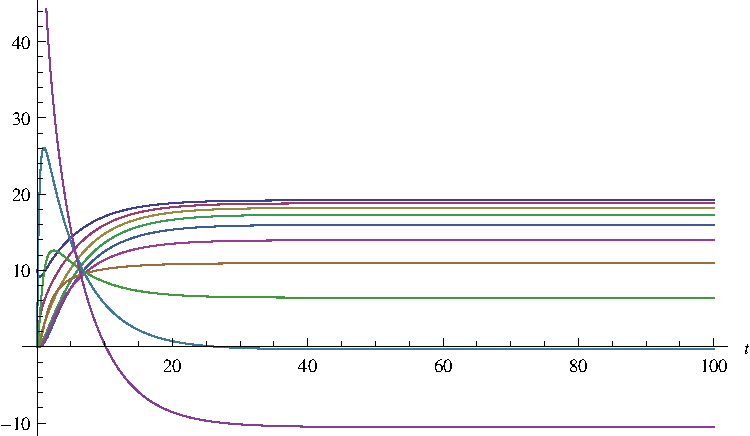
\includegraphics[width=0.8\textwidth]{individual/figures/num_sol_exp_eq_wrong}
    \caption{\label{fig:num_sol_exp_eq_wrong}Numerical solution of
    equations~\eqref{eqn:exp_equation_system_zeroth} with
\(N=10,a=1,b=0.5,c=10,d=10,S_i=0,i=1,\dotsc,N\)}
\end{figure}

\FloatBarrier
\subsection{Analysis of the expectation equations}
The expectation equations for the zeroth order transport process are a
non-closed system. In order to analyse the extent to which the neglection of the
terms relating to the probability of zero particles in
\eqref{eqn:exp_equation_system_zeroth} is a good approximation, we consider a
1-urn pure-death process with death rate \(s H(n)\), where \(n\) is the number
of particles in the urn. This simple process contains many of the difficult
features of the full process. In this case the master equation consists of the
following system:

\begin{align*}
    \diff{p_0}{t} =& s p_1\\
    \diff{p_i}{t} =& s p_{i+1} - s p_i, \quad i = 1,\dotsc,N-1\\
    \diff{p_N}{t} =& - s p_N
\end{align*}
with the initial condition
\begin{equation}
    \label{eqn:pure_death_ic}
    p_i(t=0) = \delta_{iN}.
\end{equation}
This means that there are surely \(N\) particles in the system at \(t=0\). We
are using the notation \(p_n(t)\) to denote the probability of there being \(n\)
particles in the urn at time \(t\).  Analogously to above, the deterministic
mean-field equation can be derived for this process:
\begin{equation*}
    \diff{\E{n}(t)}{t} = -s \left(1-p_0(t)\right).
\end{equation*}
As before, this equation is not closed. Therefore we cannot solve it exactly.
Assuming that \(p_0(t)\) is sufficiently smooth at \(t=0\), we can replace it
with its Taylor series around \(t=0\):
\begin{equation*}
    -s(1-p_0(t)) = -s\left(1 - \left[p_0(0) + \dot{p_0}(0)t +
    \frac{1}{2}\ddot{p_0}(0)t^2 + \dotsb \right] \right).
\end{equation*}

We have that \(p_0(0) = 0\) due to the initial condition. For the second term in
the series,
\begin{equation*}
    \dot{p_0}(0) = \left.(s(p_1)\right|_{t=0} = sp_1(0) = 0.
\end{equation*}
Similarly, for the next term,
\begin{align*}
    \ddot{p_0}(0) &= \left.\left(\diff{}{t}\dot{p_0}\right)\right|_{t=0}\\
    &= \left.\left(\diff{}{t}\left[s p_1\right]\right)\right|_{t=0}\\
    &= s^2\left(p_2(0) - p_1(0)\right) = 0.
\end{align*}
Continuing like this, we find that the derivatives of \(p_0(t)\) follow this
pattern:
\begin{equation*}
    p_0^{(i)}(t) = (-1)^i s^i \sum_{j=0}^{i-1}(-1)^j
    \binom{i-1}{j} p_{1+j}(t),
\end{equation*}
for \(i=1,\dotsc,N-1\).
Due to the initial condition \eqref{eqn:pure_death_ic}, we have that every
derivative is equal to \(0\) for \(i=1,\dotsc,N-1\). The expression for
\(i=N-1\) is
\begin{align*}
    p_0^{(N-1)}(t) &= (-1)^{N-1} s^{N-1} \left\{ p_1(t) - \binom{N-2}{1}p_2(t) +
    \dotsc \right.\\
    &\left.+ (-1)^{N-3} \binom{N-2}{N-3} p_{N-2}(t) +
    (-1)^{N-2}p_{N-1}(t)\right\}.
\end{align*}
Then we have
\begin{align*}
    p_0^{(N)}(t) &= (-1)^{N-1} s^{N-1} \left\{ \dot{p_1}(t) -
    \binom{N-2}{1}\dot{p_2}(t) +
    \dotsc \right.\\
    &\left.+ (-1)^{N-3} \binom{N-2}{N-3} \dot{p_{N-2}}(t) +
    (-1)^{N-2}\dot{p_{N-1}}(t)\right\}\\
    &= (-1)^{N-1} s^{N} \left\{ (p_2-p_1) -
    \binom{N-2}{1}(p_3-p_2) +
    \dotsc \right.\\
    &\left.+ (-1)^{N-3} \binom{N-2}{N-3} (p_{N-1} - p_{N-2}) +
    (-1)^{N-2} (p_N - p_{N-1})\right\}.
\end{align*}
Therefore
\begin{align*}
    p_0^{(N)}(0) &= (-1)^{N-1} (-1)^{N-2} s^N p_N\\
    &= (-1)^{2N-3} s^N
\end{align*}

Putting this together, we find that the Taylor series for \(-s(1-p_0)\) around
\(t=0\) is
\begin{align*}
    -s(1-p_0) = -s\left(1 - \left[ \frac{1}{N!}(-1)^{2N-3}s^N t^N + \dotsb
    \right] \right).
\end{align*}

From this we can see that \(p_0(t)\) grows like \(t^N\). Also, the first term is
scaled by a factor of \(\frac{s^N}{N!}\), which, for large \(N\) is very small.

\section{First order kinetics}
If we now assume that outflow and removal of particles obey first order
kinetics, the transition rates become
\begin{equation}
    \label{eqn:transition_rates_first_order}
    T(\V{n}|\V{n}') =
        \begin{dcases*}
            a n'_{i+1} & for \(\V{n} = \V{n}' + \V{e}_i - \V{e}_{i+1},
            i=1,\dotsc,N-1\)\\
            (a+b) n'_i & for \(\V{n} = \V{n}' - \V{e}_i + \V{e}_{i+1},
            i=1,\dotsc,N-1\)\\
            c & for \(\V{n} = \V{n}' + \V{e}_1\)\\
            d n'_N & for \(\V{n} = \V{n}' - \V{e}_N\)\\
            S_i n'_i & for \(\V{n} = \V{n}' - \V{e}_i, i=1,\dotsc,N\)\\
            0 & otherwise
        \end{dcases*}
\end{equation}
The inflow and hopping rates in remain the same as in
\eqref{eqn:transition_rates_zeroth_order}.
Therefore the only terms that change are those that correspond to removal and
outflow.

\subsection{Jump moments}
In this section we give the first two jump moments \eqref{eqn:jump_moment} for
the first-order transport problem.

\subsubsection{First jump moment}
Starting with \eqref{eqn:jump_moment} and substituting in
\eqref{eqn:transition_rates_first_order} gives
\begin{equation}
    \begin{aligned}
        a_{1i}(\V{n}) =& \sum_{\V{n}'} (n_i' - n_i) T(\V{n}' | \V{n})\\
        &= (1-\delta_{iN})(n_i + 1 - n_i)a n_{i+1}
        +  (1-\delta_{i1})(n_i - 1 - n_i)a n_i\\
        &\quad+ (1-\delta_{iN})(n_i - 1 - n_i)(a+b) n_i
        +  (1-\delta_{i1})(n_i + 1 - n_i)(a+b) n_{i-1}\\
        &\quad+ \delta_{i1}(n_1 + 1 - n_1) c\\
        &\quad+ \delta_{iN}(n_N - 1 - n_N) d n_N\\
        &\quad+ (n_i - 1 - n_i) S_i n_i\\
        &= (1-\delta_{i1})(a+b)n_{i-1} - \left[(2a+b) - \delta_{i1}a -
        \delta_{iN}(a+b) + S_i\right]n_i\\
        &\quad+ (1-\delta_{iN})an_{i+1} + \delta_{i1}c - \delta_{iN}d n_N.
    \end{aligned}
    \label{eqn:first_jump_mom_first_order}
\end{equation}
This is linear in \(\V{n}\) so we have that \eqref{eqn:linear_jump_moments}
holds. Explicitly, we have that the time evolution of the expectation of \(n_i\)
is given by
\begin{equation}
    \begin{aligned}
        \diff{\E{n_i}}{t} &= (1-\delta_{i1})(a+b)\E{n_{i-1}} - \left[(2a+b) -
        \delta_{i1}a - \delta_{iN}(a+b) + S_i\right]\E{n_i}\\
        &\quad+(1-\delta_{iN})a\E{n_{i+1}} + \delta_{i1}c - \delta_{iN}d \E{n_N},
    \end{aligned}
\end{equation}
which is equivalent to the system \eqref{eqn:exp_equation_system_first} given
below.
\begin{subequations}
    \label{eqn:exp_equation_system_first}
    \begin{gather}
        \diff{\V{\E{n}}}{t} = A \V{\E{n}}(t) + \V{b},
        \intertext{where}
        A=
        \begin{pmatrix}
            -(a+b) - S_1 & a & 0 & \dots & \dots & \dots & 0\\
            (a+b)  & -(2a+b) - S_2 & a & 0 & \dots & \dots & 0\\
            \vdots & & \ddots & \ddots & \ddots & & \vdots\\
            0 & \dots & \dots & 0 & (a+b) & -(2a+b) - S_{N-1} & a\\
            0 & \dots & \dots & \dots & 0 & (a+b) & -a -S_N - d
        \end{pmatrix}
        \intertext{and}
        \V{b}=
        \begin{pmatrix}
            c\\
            0\\
            \vdots\\
            0
        \end{pmatrix}
    \end{gather}
\end{subequations}
The coefficients \(\alpha_{1ij}\) (as in \eqref{eqn:linear_jump_moments_coeffs})
are clearly the \(i,j\) elements of the matrix \(A\), and the \(\beta_{1i}\) are the
elements of the vector \(\V{b}\).

\begin{figure}[ht!]
    \centering
    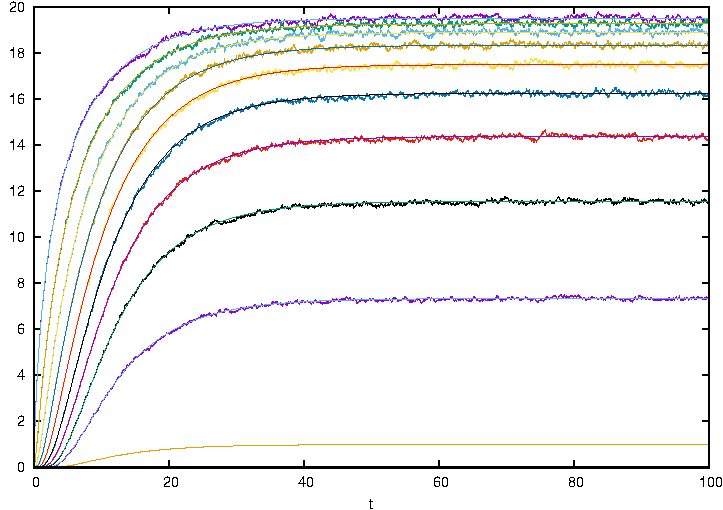
\includegraphics{individual/figures/firstorderrealisation}
    \caption{\label{fig:ex_first_order_real} Comparison between the time evolution of
the sample means of the number of particles in each urn and the mean field
approximation with first order removal kinetics.
\(N=10,a=1,b=0.5,c=10,d=10,S_i=0\).}
\end{figure}

\subsubsection{Second jump moment}
Similarly, we can find the second jump moments:
\begin{equation}
    \begin{aligned}
        a_{2i}(\V{n}) =& \sum_{\V{n}'} (n_i' - n_i)^2 T(\V{n}' | \V{n})\\
        &= (1-\delta_{iN})(n_i + 1 - n_i)^2a n_{i+1}
        +  (1-\delta_{i1})(n_i - 1 - n_i)^2a n_i\\
        &\quad+ (1-\delta_{iN})(n_i - 1 - n_i)^2(a+b) n_i
        +  (1-\delta_{i1})(n_i + 1 - n_i)^2(a+b) n_{i-1}\\
        &\quad+ \delta_{i1}(n_1 + 1 - n_1)^2 c\\
        &\quad+ \delta_{iN}(n_N - 1 - n_N)^2 d n_N\\
        &\quad+ (n_i - 1 - n_i)^2 S_i n_i\\
        &= (1-\delta_{i1})(a+b)n_{i-1} + \left[(2a+b) - \delta_{i1}a -
        \delta_{iN}(a+b) + S_i\right]n_i\\
        &\quad+ (1-\delta_{iN})an_{i+1} + \delta_{i1}c + \delta_{iN}d n_N,
    \end{aligned}
    \label{eqn:second_jump_mom_first_order}
\end{equation}
which is also linear in \(\V{n}\).

We have the following relations between the first and second jump moment
coefficients
\begin{align*}
    \alpha_{1i(i-1)} &= \alpha_{2i(i-1)}\\
    \alpha_{1ii} &= -\alpha_{2ii}\\
    \alpha_{1i(i+1)} &= \alpha_{2i(i+1)}\\
    \beta_{1i} &= \beta_{2i}
\end{align*}

\subsubsection{Mixed jump moments}
Calculating the first mixed jump moment \eqref{eqn:mixed_jump_moment_i_j}
requires slightly more effort than the regular jump moments since every
combination of relations between \(n_i\) and \(n_j\) permitted by the definition
of the rates \eqref{eqn:transition_rates_first_order} must be considered. In the
transport system, particles can only jump from urn \(i\) to urn \(j\) if \(j = i
\pm 1\), which reduces the number of terms we need to consider. However, there
are still many terms; we proceed by considering terms corresponding to each
transition type separately.
\begin{equation}
    a_{1ij}(\V{n}) = \{\text{hop left}\} + \{\text{hop right}\} +
    \{\text{inflow}\} + \{\text{outflow}\} + \{\text{removal}\}
\end{equation}

\begin{align}
    &\begin{aligned}
        \{\text{hop left}\}
        &= \delta_{(i+1)j}(1 - \delta_{iN})(n_i + 1 - n_i)(n_{i+1} - 1 -
        n_{i+1})a n_{i+1}\\
        &+ \delta_{i(j+1)}(1 - \delta_{i1})(n_i - 1 - n_i)(n_{i-1} + 1 -
        n_{i-1})a n_i\\
        &+ \delta_{ij}(1 - \delta_{iN})(n_i + 1 - n_i)(n_i + 1 - n_i)a n_{i+1}\\
        &+ \delta_{ij}(1 - \delta_{i1})(n_i - 1 - n_i)(n_i - 1 - n_i)a n_i
        \label{eqn:mixed_jump_hop_left}
    \end{aligned}\\
    &\begin{aligned}
        \{\text{hop right}\}
        &= \delta_{(i+1)j}(1 - \delta_{iN})(n_i - 1 - n_i)(n_{i+1} + 1 -
        n_{i+1})(a+b) n_i\\
        &+ \delta_{i(j+1)}(1 - \delta_{i1})(n_i + 1 - n_i)(n_{i-1} - 1 -
        n_{i-1})(a+b) n_{i-1}\\
        &+ \delta_{ij}(1 - \delta_{iN})(n_i - 1 - n_i)(n_i - 1 - n_i)(a+b) n_i\\
        &+ \delta_{ij}(1 - \delta_{i1})(n_i + 1 - n_i)(n_i + 1 - n_i)(a+b)
        n_{i-1}
        \label{eqn:mixed_jump_hop_right}
    \end{aligned}\\
    &\begin{aligned}
        \{\text{inflow}\} = \delta_{i1}\delta_{j1} (n_1 + 1 - n_1)(n_1 + 1 -
        n_1)c
        \label{eqn:mixed_jump_inflow}
    \end{aligned}\\
    &\begin{aligned}
        &\{\text{outflow}\} = \delta_{iN}\delta_{jN} (n_N - 1 - n_N)(n_N - 1 - n_N)d
        n_N
        \label{eqn:mixed_jump_outflow}
    \end{aligned}\\
    &\begin{aligned}
        &\{\text{removal}\} = \delta_{ij}(n_i - 1 - n_i)(n_i - 1 - n_i)S_i n_i
        \label{eqn:mixed_jump_removal}
    \end{aligned}
\end{align}
Summing \eqref{eqn:mixed_jump_hop_left}--\eqref{eqn:mixed_jump_removal} and
simplifying gives
\begin{equation}
    \begin{aligned}
        a_{1ij}(\V{n}) &= (a+b)(1-\delta_{i1})(\delta_{ij} -
        \delta_{i(j+1)})n_{i-1}\\
        &+ \left[ a(1-\delta_{i1})(\delta_{ij} -
        \delta_{i(j+1)}) + (a+b)(1-\delta_{iN})(\delta_{ij}-\delta_{(i+1)j}) +
    \delta_{ij}S_i \right]n_i\\
    &+ a(1-\delta_{iN})(\delta_{ij} - \delta_{(i+1)j})n_{i+1} +
    \delta_{i1}\delta_{j1}c + \delta_{jN}\delta_{iN}d n_N
    \end{aligned}
\end{equation}
It is clear from this expression that \(a_{1ij}(\V{n})\) is linear in \(\V{n}\)
and, since \(a_{1i}(\V{n})\) is also linear, we can use the simplified form of
the equation for the covariance \eqref{eqn:time_evo_covar_linear_jump_moments}.

\subsection{Variances}
We are now in a position to write down the equation governing the time
evolution of the variances for the first-order transport problem. Substituting
\eqref{eqn:first_jump_mom_first_order} and
\eqref{eqn:second_jump_mom_first_order} into
\eqref{eqn:time_evo_variance_jump_moment} gives
\begin{equation}
    \begin{aligned}
        \diff{\sigma_i^2}{t} &= (1-\delta_{i1})(a+b)\E{n_{i-1}} +
        \left[(2a+b) - \delta_{i1}a - \delta_{iN}(a+b) + S_i\right]\E{n_i}\\
        &\quad+ (1-\delta_{iN})a\E{n_{i+1}} + \delta_{i1}c + \delta_{iN}d \E{n_N}\\
        &\quad+ 2 \sum_{j=1}^N \alpha_{1ij} \sigma(n_i,n_j)
    \end{aligned}
    \label{eqn:time_evo_variance_first_order}
\end{equation}
So, in general, the variance of \(n_i\) can depend on the covariances between
\(n_i\) and all other \(n_j\). This suggests that we derive the corresponding
equation for the covariances, which we do below.

\subsubsection{No correlation}
If we make the assumption that there is no covariance between any \(n_i, n_j,
i\neq j\), then the equation for the variance simplifies to
\begin{equation}
    \begin{aligned}
        \diff{\sigma_i^2}{t} &= (1-\delta_{i1})(a+b)\E{n_{i-1}} +
        \left[(2a+b) - \delta_{i1}a - \delta_{iN}(a+b) + S_i\right]\E{n_i}\\
        &\quad+ (1-\delta_{iN})a\E{n_{i+1}} + \delta_{i1}c + \delta_{iN}d \E{n_N}\\
        &\quad+ 2 \alpha_{1ii} \sigma_i^2.
    \end{aligned}
    \label{eqn:time_evo_variance_first_order_no_corr}
\end{equation}
This system is only coupled with the other variances, as opposed to
\eqref{eqn:time_evo_variance_first_order} which also depends on the covariances.

\begin{figure}[ht!]
    \centering
    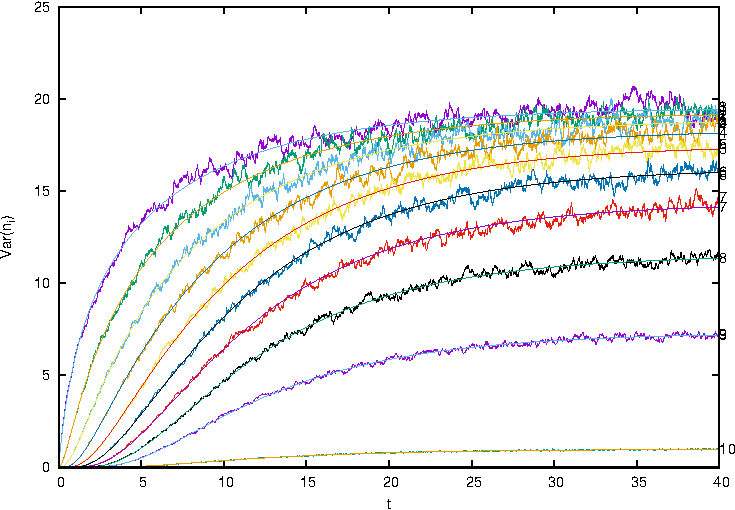
\includegraphics{individual/figures/variance_first_order_no_corr}
    \caption{\label{fig:variance_first_order_no_corr} Comparison of a sample
average of the variance (from 5000 runs) and the analytical prediction under the
assumption zero correlation between urns, with parameters \(N=10,a=1,b=0.5,c=10,d=10,S_i=0\).}
\end{figure}

\subsection{Covariances}
We can now solve \eqref{eqn:time_evo_covar_linear_jump_moments} subject to the
initial conditions
\begin{equation*}
    \sigma_{ij}(t=0) = 0, \text{ for } i,j=1,\dotsc,N.
\end{equation*}
An example solution, given as a matrix plot, is shown in
figure~\ref{fig:ex_covariance_first_order_exact}. For comparison, the
corresponding plot generated from the sample covariances of 9999 Gillespie runs
for the same parameters is shown in
figure~\ref{fig:ex_covariance_first_order_gillespie}.

\todo{plot this in a less terrible way}
\todo{include table of numerical values}

\begin{figure}
    \centering
    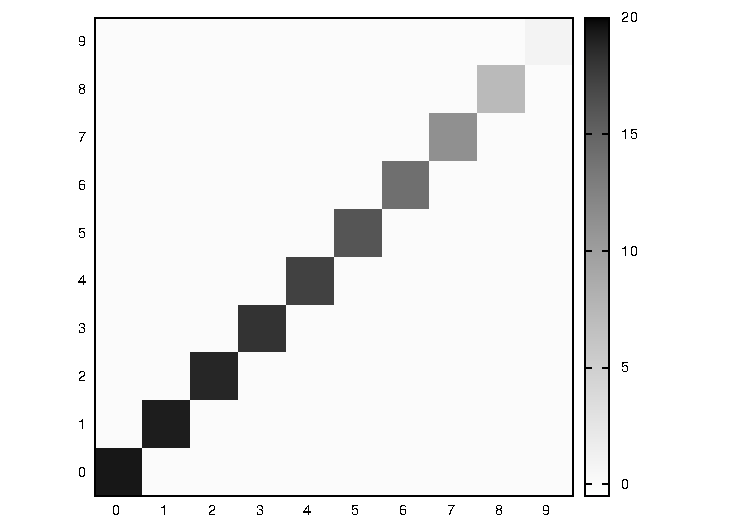
\includegraphics{individual/figures/covariance_exact_40}
    \caption{\label{fig:ex_covariance_first_order_exact}Exact covariance matrix for
parameters \(N=10,a=1,b=0.5,c=10,d=10,S_i=0\)}
\end{figure}
\begin{figure}
    \centering
    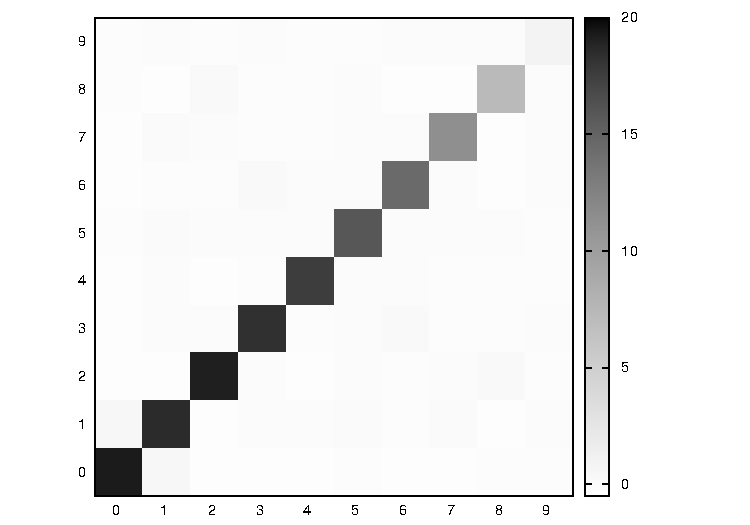
\includegraphics{individual/figures/covariance_gillespie_40}
    \caption{\label{fig:ex_covariance_first_order_gillespie}Sample covariance
matrix (from 9999 runs) for parameters \(N=10,a=1,b=0.5,c=10,d=10,S_i=0\)}
\end{figure}

The exact covariance equation \eqref{eqn:time_evo_covar_linear_jump_moments} is
solved numerically using \texttt{Mathematica}. The numerical solution has very
small (\(\sim 10^{-9}\) --- many orders of magnitude smaller than the Gillespie)
off-diagonal elements which are most likely numerical artefacts.

\FloatBarrier
\section{Todo/problems}
\begin{itemize}
    \item Show analytically that \(\sigma_{ij} = 0\) when \(i \neq j\)
    \item Write up exact solution of 1 urn 1st order death process
    \item Unbiased transport --- keep biased everywhere except for when solving
        the linear system?
    \item Update plots --- consistent colours, line labels
\end{itemize}
